\documentclass{article}
\usepackage{tikz}
\usepackage{subfig}
\usetikzlibrary{circuits.ee.IEC}
\usetikzlibrary{circuits.logic.US}
\begin{document}

    \centering
    {
        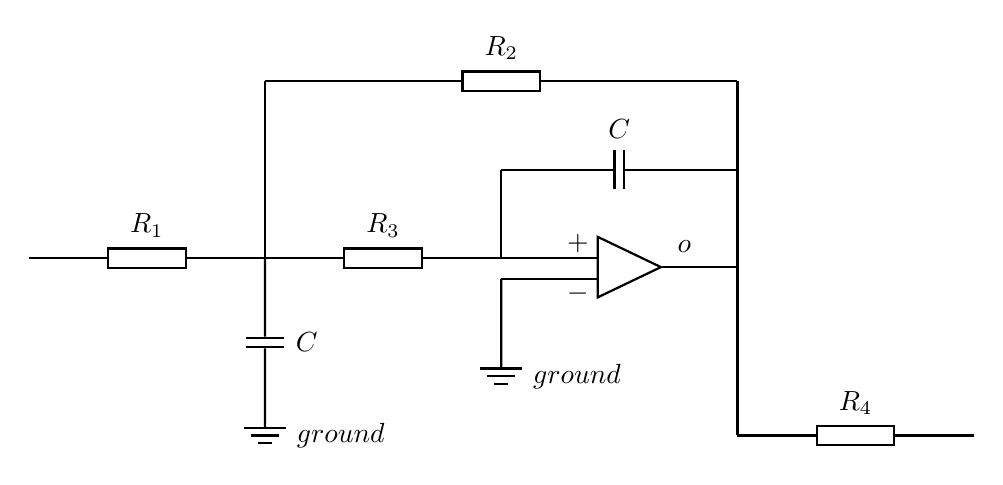
\begin{tikzpicture}[thick,circuit ee IEC,thick,circuit logic US,scale = 0.75]
           \node at (0,-6)  [ground={info={$ground$}},huge circuit symbols,point down](n1) {};
           \draw (0,-3) to [resistor={info'={$R_1$}}] (-4,-3){} ;
            \draw (0,0) to [resistor={info={$R_2$}}] (8,0) ;
            \draw (8,0) to (8,-6);
            \draw (4,-1.5) to [capacitor={info={$C$}}] (8,-1.5);
            \draw (0,0) to (0,-3);
            \draw (0,-3) to [capacitor={info={$C$}}] (n1);
            \draw (0,-3) to [resistor={info={$R_3$}}] (4,-3);
            \node at (6,-3.15) [huge  circuit symbols,buffer gate] (oa) {};
            \draw (8,-6) to [resistor={info={$R_4$}}] (12,-6);      
            \node at (4,-5) [ground={info={$ground$}},huge circuit symbols,point down](n2) {};
          	 \draw (4,-3.35) to (n2);
          	 \draw (4,-1.5) to (4,-3);
          	 \draw (6.7,-3.15) to  (8,-3.15); \node at (7.1,-2.8) {$o$};
          	 \draw (4,-3.35)to (5.62,-3.35); \node at (5.3,-3.6) {$-$};
             \draw (4,-3) to (5.62,-3); \node at (5.3,-2.75){$+$};
        \end{tikzpicture}
    }


\end{document}